\documentclass[11pt,a4paper]{article}

\usepackage[T1]{fontenc}
\usepackage[utf8]{inputenc}
\usepackage{lmodern}
\usepackage{microtype}
\usepackage[margin=1in]{geometry}
\usepackage{amsmath}
\usepackage{booktabs}
\usepackage{tabularx}
\usepackage{graphicx}
\usepackage{enumitem}
\usepackage[round,authoryear]{natbib}
\usepackage[hidelinks]{hyperref}
\usepackage{url}

\setlist{itemsep=2pt,topsep=4pt}

\title{Transfer and Re-checking of Learned Rules\\Across Levels in ARC-AGI-3}
\author{}
\date{November 2026}

\begin{document}

\maketitle

\begin{abstract}
An agent that learns the rules of a game while playing it must decide, at every new level, how far to trust what it learned on the last one. We study this decision in ARC-AGI-3, an interactive benchmark whose levels deliberately introduce new mechanics. Our agents use no pretraining and no language model: they explore a graph of game states and keep simple statistics about which actions change the screen. All comparisons are paired by seed, and every experiment was preceded by written predictions.

We report four findings. First, carrying action statistics across levels helps on average: on six games that reach a second level, it used fewer actions than starting fresh in 36 of 51 paired runs (sign test $p = 0.002$). Second, it fails in a specific, repeatable way: when the rule that matters on the new level was learned from only a handful of tries, the agent keeps a wrong ranking and often never finishes the level. Third, re-checking old rules repairs this failure, but re-checking every thinly supported rule costs about what transfer saves. Both patterns replicate in a second agent with roughly twice the score, built by combining ours with a published graph explorer. Fourth, in procedurally generated games where we control the cause, the best strategy switches with the number of irrelevant object kinds: re-checking wins when there are few, trusting old knowledge when there are many.

A rule suggested by the generated games, re-checking only thin rules that have shown some effect, was as safe as starting fresh and repaired the original failure on fresh seeds, at no measurable cost. Its speed advantage over starting fresh, strong on the seeds where it was developed (68\% of pairs, $p = 0.004$), did not reach our pre-set bar on new seeds (59\%, $p = 0.11$). We report it as a safety result, not a speed result.
\end{abstract}

\section{Introduction}

Any system that learns from experience and carries what it learned into a new situation faces the same question: which of its old beliefs still hold? Trusting everything is fast but brittle. Re-testing everything is safe but throws away the point of having learned. People handle this without much thought. We do not check that a chair will hold our weight, but we do test the ice before walking onto a frozen lake. Current learning systems mostly do not make that distinction.

ARC-AGI-3 makes the question concrete. Its games come without instructions, and each level of a game adds or changes mechanics \citep{arcprize2026}. An agent that has worked out level~1 arrives at level~2 with useful knowledge and some knowledge that is now wrong, and it is scored on how few actions it needs. Spending actions to re-check old beliefs is therefore a visible cost, not a hidden one.

We study this trade-off with deliberately simple agents. They build a graph of the game states they have seen, and they count how often each kind of action, including clicks on each kind of object, changes the screen. Those counts decide what the agent tries first. Because the agents have no learned representations, every carried-over belief can be inspected, and every failure can be traced to the belief that caused it.

Our contributions are:
\begin{enumerate}
  \item \textbf{A measured benefit and a measured failure.} Carrying statistics across levels saves actions on average, and fails when a decisive rule rests on thin evidence (Section~\ref{sec:transfer}).
  \item \textbf{A replication in a stronger agent.} We reproduce a published graph explorer, find and fix a bug that disables its error recovery offline, and combine it with our agent. The combination roughly doubles the score of either parent, and the transfer findings hold inside it (Sections~\ref{sec:combined} and~\ref{sec:replication}).
  \item \textbf{A map of the trade-off.} Re-checking repairs the failure but cancels the benefit. A procedural game generator shows why: whether re-checking pays depends on how many thinly supported, irrelevant kinds share the screen with the decisive one (Section~\ref{sec:generated}).
  \item \textbf{A rule that keeps the safety.} Re-checking only thin rules that have shown some effect was as safe as starting fresh on new seeds and fully repaired the original failure. Its speed advantage did not survive our pre-set test (Section~\ref{sec:recheck}).
\end{enumerate}

A note on method. We wrote down predictions before every experiment and report them all, including the many we got wrong (Appendix~\ref{app:predictions}). We also say where a design was changed after a pilot, and where an idea was tested on the same data that suggested it.

\section{Related work}

\paragraph{ARC-AGI-3 agents.} The closest prior agent is the training-free graph explorer of \citet{rudakov2025}. It segments frames into single-colour objects, masks status bars, ranks click targets by visual salience and walks a state graph to the nearest untested action; it placed third on the private leaderboard of the ARC-AGI-3 preview. Our explorer rediscovers much of this design, and we build on their code directly in Section~\ref{sec:combined}. The preview winner, StochasticGoose \citep{smit2025}, trains a small convolutional network to predict whether an action will change the frame and steers exploration towards those that will; our action statistics are a much cruder, count-based version of the same signal. Current top scores in the ARC Prize 2026 Kaggle competition come from harnesses built around small open language models \citep{metir2026}, far stronger than anything studied here.

\paragraph{Learned priorities across levels.} A Stanford course project \citep{bookman2026} replaced Rudakov et al.'s fixed salience ranking with learned ones, several of which carry weights across levels. It evaluated one game (vc33) with three runs, and noted that overfitting to level~1 can harm later levels, without measuring when this happens or what repairs it. That gap is the subject of this paper.

\paragraph{Object-based models and theory learning.} Learning action effects per object type goes back at least to object-oriented MDPs \citep{diuk2008}. Schema Networks showed zero-shot transfer across Breakout variants \citep{kansky2017}, and EMPA learns game theories by Bayesian inference and approaches human learning speed on 90 Atari-style games \citep{tsividis2021}. These systems model far more than ours does. We use a minimal model on purpose, so that the effect of trusting or re-checking each belief can be isolated.

\paragraph{Re-checking beliefs.} Comparing an old-plus-new model against a new-only model by Bayes factor is standard model comparison, and the value of re-testing uncertain beliefs is a familiar theme in exploration under uncertainty. We claim no novelty for these tools, only for the paired measurement of how they trade off against transfer in this setting.

\section{Setting}

We use the 25 public ARC-AGI-3 games shipped with the official toolkit (arc-agi 0.9.9), played offline. A game has 6 to 10 levels, a $64 \times 64$ frame of 16 colours, and up to seven actions, one of which is a click at a chosen cell. No rules or goals are given.

Each level is scored against a human baseline for that level, and the efficiency ratio is squared:
\begin{equation}
  s_\ell = \min\left(115,\; 100 \cdot \left(\frac{h_\ell}{a_\ell}\right)^{2}\right),
\end{equation}
where $h_\ell$ is the human baseline and $a_\ell$ the agent's actions on level~$\ell$. An unfinished level scores zero. A game's score is the level-weighted mean, capped at the weighted share of completed levels, and the overall score is the mean over games. Our implementation matched the toolkit's own calculator on all 600 full-game runs we checked. Because of the square, an agent that needs ten times the human's actions earns one point out of a hundred, so the score is dominated by how quickly levels are solved, not by how many.

Every run had a budget of 10,000 actions per game. Resets after a game-over were not counted as actions, for all agents alike. The transfer experiments focus on the six games where some agent ever cleared level~2 within the budget: cd82, dc22, lf52, lp85, tu93 and vc33.

\section{Agents}

\subsection{The rule agent}

The agent treats each distinct frame as a node in a graph and each action as an edge. In every new state it lists the available actions, with clicks restricted to the centre of each same-coloured connected region (at most 80, smallest first). It tries untried actions in the current state, and otherwise walks the graph to the nearest state that still has promising untried actions. Actions that led to a game-over are avoided.

Three additions turn this explorer into a learner:
\begin{enumerate}
  \item \textbf{Counter masking.} A probe of all 25 games showed that 22 display a step counter: a bar on one edge that changes one or two cells on every action. A row or column where small changes keep landing on new cells, on most steps and under different actions, is masked out of the state. If the graph is exhausted without a win, the mask is dropped for that level.
  \item \textbf{Action kinds.} A click's kind is the colour and bounding-box size of the object clicked; a plain action is its own kind.
  \item \textbf{Effect statistics.} For each kind, the agent counts tries and how many changed the masked frame. Untried actions are ranked by the estimated chance of an effect, $(c + 1)/(n + 2)$, with never-tried kinds first. Nothing is ever ruled out, so the search remains complete.
\end{enumerate}

\subsection{What happens at a new level}

The variants differ only in what they do with the statistics when a level is cleared (Table~\ref{tab:variants}). Up to that moment they are the same program and, with the same seed, take identical actions.

\begin{table}[ht]
\centering
\caption{The variants and what each does when a level is cleared.}
\label{tab:variants}
\small
\begin{tabularx}{\textwidth}{@{}lX@{}}
\toprule
Variant & At each new level \\
\midrule
Reset & Forget everything: statistics and masks \\
Transfer & Keep everything \\
Surprise check & Keep, but re-try every carried kind twice early; drop a kind's old evidence when the new level contradicts it (log Bayes factor of new-only over old-plus-new above 2) \\
Drop only & Keep, drop contradicted evidence, but never re-try on purpose \\
Selective & As surprise check, but re-try only kinds with fewer than 10 earlier tries \\
Value of information & Re-try a carried kind only if its plausible range (mean $\pm$ 2 sd) overlaps another kind in the same state \\
Effective-thin & Re-try only kinds with fewer than 10 earlier tries that changed the frame at least once \\
\bottomrule
\end{tabularx}
\end{table}

\subsection{A published explorer and a combined agent}
\label{sec:combined}

To test our findings in a stronger agent, we ran Rudakov et al.'s explorer unmodified, through a thin wrapper for the offline toolkit. In doing so we found that its main loop, after an internal error, asks for the graph to be rebuilt but cancels that request on the next step. Offline, where a reset after game-over can make a tested action appear to behave differently, this leaves the agent repeating one action for the rest of the game: a median of 9,088 errors per game, and level~1 cleared on only 6 of 25 games. Keeping the rebuild request for one step, as the code's own log message intends, restores normal behaviour.

With that fix, their explorer scores 0.33 (three seeds: 0.23, 0.53, 0.22) against 0.27 for our rule agent, but clears level~1 on only 10 games to our 15--16. The two agents succeed on different games, so we combined them: our agent plus their shape-based status-bar detector and their salience ranking, used only as the starting order of never-tried kinds. The combined agent scores 0.60 (0.72, 0.43, 0.65) and clears level~1 on 17 games on every seed. Section~\ref{sec:replication} repeats the transfer experiments inside it.

\section{Protocol}

\paragraph{Pairing.} Because the variants are identical until level~1 is cleared, two variants run with the same seed reach level~2 at the same moment, in the same state. We checked this in every experiment and found no mismatch. The seed only controls the agent's random tie-breaks; the games are fixed. Any difference on level~2 is therefore caused by what the variant carried over.

\paragraph{Measures.} For each variant we count the game-seeds on which level~2 was cleared within the budget (safety), and, over pairs where both the variant and Reset cleared it, the share in which the variant used fewer level-2 actions, with a one-sided sign test (speed). We also report the geometric mean of the action ratio. Most experiments use 10 seeds on the six games above, giving 60 game-seeds.

\paragraph{Predictions.} Before each experiment we wrote numbered predictions with explicit thresholds, dated, into a log file kept with the code, and we score them as written. Appendix~\ref{app:predictions} lists all of them. Two departures from this are worth stating here. In the generated games (Section~\ref{sec:generated}), a pilot showed the first design could not test what it was meant to; we withdrew those predictions unscored, changed the design and wrote new ones before the main run. And the effective-thin rule was suggested by the generated games and first tested on the same ARC seeds as the earlier variants, so we confirmed it on ten fresh seeds with criteria fixed in advance (Section~\ref{sec:recheck}).

\paragraph{Compute.} Everything ran on a four-core laptop CPU. A full sweep of 25 games and three seeds takes under an hour for our agents; the generated games run in seconds.

\section{Results on the ARC games}

\subsection{Transfer helps on average and fails on thin evidence}
\label{sec:transfer}

On our rule agent, Transfer used fewer level-2 actions than Reset in 36 of 51 paired runs ($p = 0.002$), about 11\% fewer on average (geometric-mean ratio 0.89). It was also less safe: it cleared level~2 on 52 of 60 game-seeds, against 58 for Reset, and almost all of the difference came from one game, lf52, where Transfer cleared level~2 on only 3 of 10 seeds.

The lf52 failure has a simple cause. On level~1 the agent learned that clicks on $1 \times 1$ objects change the frame 58\% of the time, from 48 tries, and that clicks on $4 \times 4$ objects of one colour do so 43\% of the time, from just 5. On level~2 those larger objects are what matters and work about 90\% of the time. A fresh agent tries every kind early and finds this out. The transferring agent ranks the many small objects first in every new state, spends its budget on them, and its new evidence never contradicts the old ranking strongly enough to overturn it. The failure is not a wrong rule so much as a weakly supported ranking that is never re-examined.

\subsection{Replication in the combined agent}
\label{sec:replication}

We repeated the experiment, unchanged, inside the combined agent of Section~\ref{sec:combined}. Transfer again beat Reset more often than not (34 of 53 pairs, $p = 0.03$), again cleared level~2 less often (54 against 58), and again failed on lf52 (5 of 10 seeds against Reset's 9). One thing changed: the average saving almost vanished (geometric-mean ratio 0.99, against 0.89). The salience ranking now supplies, from the first frame, much of what transfer used to carry over. All five predictions for this replication held.

\subsection{Re-checking}
\label{sec:recheck}

Table~\ref{tab:main} shows every variant on both agents. Three patterns are consistent.

\begin{table}[ht]
\centering
\caption{Level~2 on six games, seeds 0--9 unless stated. ``Beat Reset'' is the share of pairs in which the variant needed fewer level-2 actions; $p$ is a one-sided sign test.}
\label{tab:main}
\small
\begin{tabular}{@{}llrrrr@{}}
\toprule
Agent & Variant & \shortstack[r]{Level 2 cleared\\(of 60)} & Beat Reset & $p$ & \shortstack[r]{lf52 cleared\\(of 10)} \\
\midrule
Rule agent & Reset & 58 & -- & -- & 9 \\
 & Transfer & 52 & 71\% & 0.002 & 3 \\
 & Drop only & 52 & 71\% & 0.002 & 3 \\
 & Surprise check & 57 & 52\% & 0.45 & 10 \\
 & Selective & 55 & 55\% & 0.29 & 9 \\
 & Value of information & 57 & 53\% & 0.39 & 9 \\
 & Effective-thin & 59 & 68\% & 0.004 & 9 \\
\midrule
Rule agent, & Reset & 56 & -- & -- & 9 \\
\quad seeds 10--19 & Transfer & 55 & 73\% & 0.001 & 5 \\
 & Selective & 53 & 50\% & 0.56 & 7 \\
 & Effective-thin & 57 & 59\% & 0.11 & 10 \\
\midrule
Combined & Reset & 58 & -- & -- & 9 \\
 & Transfer & 54 & 64\% & 0.03 & 5 \\
 & Drop only & 51 & 57\% & 0.20 & 5 \\
 & Surprise check & 56 & 56\% & 0.21 & 8 \\
 & Selective & 57 & 57\% & 0.17 & 9 \\
 & Value of information & 54 & 58\% & 0.17 & 9 \\
 & Effective-thin & 52 & 54\% & 0.34 & 5 \\
\bottomrule
\end{tabular}
\end{table}

First, noticing a contradiction is not enough. Drop only does fire on lf52, discarding two to five old rules per seed, and still fails it as often as Transfer. By the time the contradiction is visible, the budget has gone. Only variants that go and look early repair lf52.

Second, looking early has a price. Every variant that re-checks broadly is about as safe as Reset and loses Transfer's speed. The value-of-information variant was meant to re-check only where the answer could change a decision, but its logs show that it re-checked nearly everything: most carried kinds rest on a few tries, so their plausible ranges are wide and nearly always overlap something.

Third, the effective-thin rule, which came out of the generated games in Section~\ref{sec:generated}, was the only variant on the rule agent that was both as safe as Reset and clearly faster on seeds 0--9. On ten fresh seeds it remained safe (57 against 56), repaired lf52 on all ten seeds and cost nothing on lp85, the game where earlier re-checking variants paid most. Its speed advantage fell to 59\% of pairs ($p = 0.11$), just under the 60\% we had fixed in advance, so by our own criterion the speed claim is not confirmed. On the combined agent it did not help at all. There, level~1 of lf52 is cleared so quickly that the decisive kind is often clicked only once or twice and on five of ten seeds never changes the frame, so the rule trusts it as useless. This explains three of the five failures; the other two remain unexplained.

\section{Controlled games}
\label{sec:generated}

The ARC results rest on six games, and the failure on one. To test the explanation rather than illustrate it, we built a generator of small games that the same agent plays through the same interface, unchanged.

\subsection{Design}
\label{sec:gendesign}

Each generated game has two levels on a $64 \times 64$ frame and accepts only clicks. Objects are filled rectangles; an object's kind is its colour and size, which is exactly the agent's own notion of kind. A small indicator near the top-left cycles through four colours. Within a level each kind plays one role:
\begin{itemize}
  \item \textbf{Key} (2 objects): a click removes the object; removing both clears the level.
  \item \textbf{Decoy}: every click advances the indicator. It always does something and never helps.
  \item \textbf{Half}: every second click on the same object advances the indicator.
  \item \textbf{Inert} (10 objects): nothing happens.
\end{itemize}

We vary what changes between levels. In \textsc{stable} the roles stay the same. In \textsc{promoted\_half} the old half-decoy becomes the key, which is the lf52 pattern. In \textsc{promoted\_inert} the key is a kind that did nothing on level~1. In \textsc{new} it is a kind never seen before. Layouts, colours and sizes are drawn from a seeded generator, and a validation script checks that every game is deterministic, solvable in four clicks and free of overlapping or touching objects.

A pilot with 4 or 12 decoys and 3 inert objects found that Transfer was slower than Reset even in \textsc{stable}. The cause is instructive: the agent learns which actions change the screen, not which make progress, and a decoy changes the screen every time while the key is clicked only twice before it is gone. With decoys in every game, the first design could not show transfer helping at all. We withdrew its predictions unscored and reran with 0 or 6 decoys and 10 inert objects.

\subsection{When carried knowledge helps}

Across 200 games, Transfer was faster than Reset on all 25 \textsc{stable} games without decoys (median ratio 0.38) and when the key was new (0.57). It was slower whenever decoys were present and the key had changed or stayed the same (ratios 1.43--1.55), and always slower when the key had done nothing on level~1 (2.0--3.5). Carried knowledge helps when it ranks the decisive kind high and hurts when kinds that merely do something outrank it. That is the lf52 mechanism, now reproduced on demand.

The selective variant gave a result we did not predict. With decoys present it was about five times faster than Reset (ratios 0.18--0.21). The key is used up when it works, so it is always the thinly supported kind; re-checking thin kinds first therefore means trying the key first.

\subsection{The flip}

That raised an obvious question: why did selective re-checking not shine on the ARC games? There, dozens of kinds rest on a few tries each, so being thinly supported no longer singles out anything. We tested this by adding $k$ irrelevant kinds, each a single inert object, using a denser layout to fit up to 64 of them, with 100 games per condition and $k$ (1,000 games).

\begin{figure}[ht]
\centering
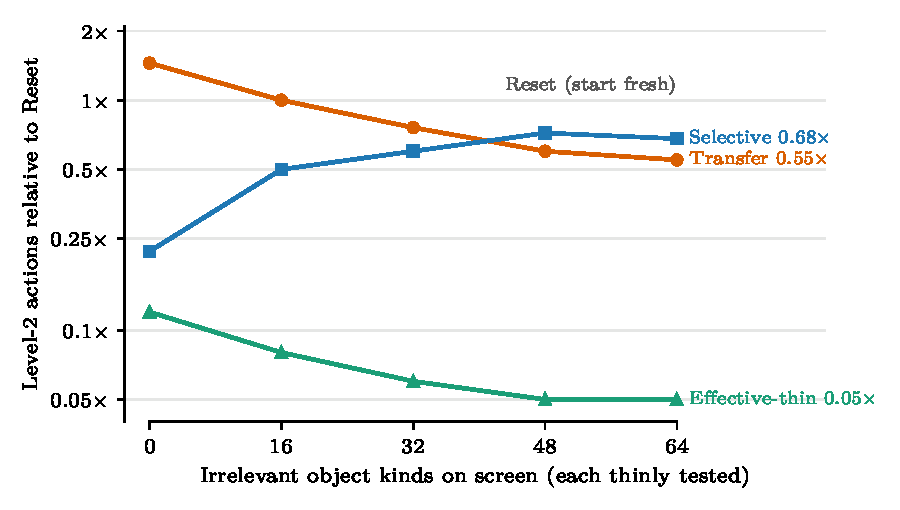
\includegraphics[width=0.85\textwidth]{figure1}
\caption{As irrelevant kinds multiply, the better of Transfer and Selective flips. Generated games, \textsc{stable} condition, 6 decoys, 100 games per point; median level-2 actions relative to Reset (log scale). 1,000 games in total; \textsc{promoted\_half} gives the same shape (Appendix~\ref{app:predictions}).}
\label{fig:flip}
\end{figure}

Re-checking never fell behind Reset, but its edge shrank from about five times to about one and a half (Figure~\ref{fig:flip}). Transfer improved steadily, because it already knows which of the many kinds do nothing while Reset must try them. Between 32 and 48 irrelevant kinds the better of the two flips. The ARC games, with their dozens of rarely clicked kinds, sit on the right of this figure, which is where we found Transfer ahead and broad re-checking costly.

\subsection{Re-checking only what has worked}

The figure suggests a sharper rule. The key is thinly supported and does something; irrelevant kinds are thinly supported and do nothing. The effective-thin variant re-checks only thin kinds that changed the frame at least once. On the 1,000 dense games it needed 0.05--0.12 of Reset's actions and was faster on 97--100\% of games in every condition. That margin is partly built in: the generator's key always is a thin kind with an effect. Where it is not, in \textsc{promoted\_inert}, the rule trusts the old ``does nothing'' and is as slow as Transfer (2.0--3.6 times Reset). Section~\ref{sec:recheck} reports how it fared on the ARC games.

\section{Discussion and limitations}

The central result is not a new agent but a description of a trade-off. Knowledge carried from one level to the next is worth something, and its main failure comes from beliefs formed on little evidence that are never looked at again. Noticing a contradiction in passing does not help, because by then the damage is done; going back to check does help, but each check costs actions, and on games with many rarely tried kinds the checks add up to more than transfer saved. The generated games show that this is not a quirk of six ARC levels: the same mechanism appears on demand, and which side of the trade-off wins depends on how crowded the screen is with thinly tested, irrelevant kinds.

A second, more general point came out of the pilot. Our agent measures whether an action changes the screen, not whether it makes progress. On the ARC games this distinction was hidden, but in a controlled game with a few busy decoys it decides everything. Agents that rank actions by surprise, novelty or change face the same issue; a learned progress signal would probably matter more than any re-checking rule.

The effective-thin rule deserves a measured claim. On fresh seeds it was as safe as starting fresh, removed the lf52 failure completely and cost nothing where other re-checking variants were expensive. That is a useful property. Whether it is also faster than starting fresh is unresolved: strong on the seeds where the idea was developed, short of our threshold on new ones. It also bets that the decisive kind has shown some effect before, and it fails, as the generated games predict, when that is not so. On the combined agent that happened often enough to cancel its benefit.

The limitations are substantial:
\begin{itemize}
  \item \textbf{Scale.} The transfer story rests on six games, and its failure case on one. The generated games broaden the evidence but are tiny, with two levels and one decisive kind.
  \item \textbf{Hand-made vocabulary.} The agent learns only within categories we chose: objects defined by colour and size, effects defined as any change of the screen. A general learner would have to discover such categories itself.
  \item \textbf{Weak agents.} Our best agent scores 0.60 out of 100. Language-model harnesses on Kaggle score near 56. Whether the trade-off looks the same inside such systems, where carried knowledge lives in context or weights rather than counts, is open.
  \item \textbf{Many variants on the same data.} Seven variants were compared on the same seeds. We confirmed the one positive result on fresh seeds, and it only partly survived.
  \item \textbf{A known confound.} Actions taken while walking to a planned state also update the effect statistics. We left this in place so that every variant stayed comparable.
\end{itemize}

\section{Conclusion}

An agent that learns rules while playing should carry them forward, but not blindly. In ARC-AGI-3, transfer between levels saves actions on average and fails when a decisive belief was formed on too little evidence. Re-checking fixes the failure only if the agent goes and looks early, and looking costs what transfer saved, unless the agent can tell which thin beliefs are worth looking at. Our best answer so far, re-checking only thin rules that have shown an effect, buys safety at no measurable cost but not, on fresh data, a clear gain in speed. The deeper problem it points to is that our agents cannot tell change from progress, and a learner that could would face this trade-off on much better terms. The code, logs and prediction record are released with this paper so that others can check these results and build on them.

\appendix

\section{Prediction record}
\label{app:predictions}

Every experiment was preceded by dated, numbered predictions with explicit thresholds. Of 57 scored predictions, 31 held in full and 3 held in part. The first generated-game design's 5 predictions were withdrawn unscored after the pilot described in Section~\ref{sec:gendesign}. Misses were mostly overestimated effect sizes, plus two wrong diagnoses: we expected the explorer to fail mainly through counter-driven state explosion, and the surprise check to fail on lf52.

\begin{table}[ht]
\centering
\caption{Predictions by experiment.}
\label{tab:predictions}
\small
\begin{tabular}{@{}lrrrr@{}}
\toprule
Experiment & Predictions & Held in full & Held in part & Missed \\
\midrule
Baselines & 5 & 3 & 1 & 1 \\
Rule agent, Reset vs Transfer (3 seeds) & 5 & 3 & 0 & 2 \\
Surprise check (3 seeds) & 5 & 3 & 0 & 2 \\
Re-checking ablation, rule agent (10 seeds) & 4 & 1 & 2 & 1 \\
Combined agent & 5 & 3 & 0 & 2 \\
Replication in combined agent & 5 & 5 & 0 & 0 \\
Value of information & 5 & 1 & 0 & 4 \\
Generated games, main design & 5 & 2 & 0 & 3 \\
Generated games, irrelevant kinds up to 16 & 4 & 2 & 0 & 2 \\
Generated games, dense, up to 64 & 4 & 2 & 0 & 2 \\
Effective-thin & 5 & 2 & 0 & 3 \\
Effective-thin, fresh seeds & 5 & 4 & 0 & 1 \\
\midrule
Total & 57 & 31 & 3 & 23 \\
\bottomrule
\end{tabular}
\end{table}

Figure~\ref{fig:flip} shows the \textsc{stable} condition. In \textsc{promoted\_half} the median ratios to Reset at $k = 0, 16, 32, 48$ and 64 were 1.58, 1.06, 0.80, 0.64, 0.57 for Transfer; 0.21, 0.47, 0.55, 0.60, 0.72 for Selective; and 0.12, 0.08, 0.06, 0.05, 0.06 for Effective-thin.

\section{Reproducibility}

All runs used the offline toolkit arc-agi 0.9.9 with Python 3.13 on Windows, with \texttt{PYTHONHASHSEED} fixed to 0, because the published explorer iterates over sets of strings. The agent seed controls only random tie-breaks; every game was run with game seed 0. Repeated runs reproduced earlier results exactly wherever we checked. The published explorer was run unmodified from its repository; our wrapper changes only the plumbing and the one re-initialisation step described in Section~\ref{sec:combined}, and can be switched back to the original behaviour.

\bibliographystyle{plainnat}
\bibliography{references}

\end{document}
